% M1 writing brief: formulas, parameters, construction, results, goals.
% Build in Reports/M1: pdflatex M1_writing_brief.tex (twice)
\documentclass[11pt,a4paper]{article}
\usepackage[margin=2.1cm]{geometry}
\usepackage{newtxtext,newtxmath}
\usepackage{amsmath,bm}
\usepackage{booktabs,tabularx,array,multirow}
\usepackage{graphicx,float,caption}
\usepackage{enumitem,xcolor}
\usepackage{algorithm}
\usepackage[noend]{algpseudocode}
\usepackage[hidelinks]{hyperref}
\algrenewcommand\algorithmicrequire{\textbf{Input:}}
\algrenewcommand\algorithmicensure{\textbf{Output:}}
\setlist{itemsep=1pt,topsep=3pt}
\captionsetup{font=small}
\renewcommand{\arraystretch}{1.18}
\newcolumntype{Y}{>{\raggedright\arraybackslash}X}
\newcommand{\Wb}{\overline W}
\newcommand{\say}[1]{\par\smallskip\noindent\textcolor{teal!70!black}{\textit{Writing note:} #1}\par\smallskip}

\title{\textbf{Model 1 Writing Brief}\\[2pt]\large Coupled vegetation--water--sand dynamics (Task 1)}
\author{Source of every number: \texttt{Results/v7/model1/} (run of \texttt{Code/v7\_model1.py})}
\date{2026-11-11}

\begin{document}
\sloppy
\maketitle

\noindent This brief collects what you need to write the Model 1 section of the paper:
the goal, how the model is built, every formula with its meaning, parameter values,
the results with numbers, and what the results do and do not allow you to claim.
All values are copied from the result tables; figure files are in \texttt{Figures/M1/}.
Units: $V$ is in percentage points of a cover proxy, $M$ in mm, irrigation in mm/yr on the
treated area ($1$ mm $=10$ m$^3$/ha).

\tableofcontents

% =====================================================================
\section{Goal and what we achieved}

Task 1 asks for a coupled dynamic model of vegetation cover and effective soil moisture on
a representative section of the desert margin, using real data, and for the factors that drive them.

\begin{table}[H]\centering\small
\begin{tabularx}{\textwidth}{@{}p{3.4cm}YY@{}}
\toprule
Requirement & How Model 1 meets it & Evidence \\
\midrule
Representative section (width tens of m to km, length tens to hundreds of km) &
Yutian--Minfeng southern margin of the Taklimakan, centre line through windows CON1--CON4, length 127.95 km, assumed width 1 km &
\texttt{section\_definition.json} \\
Coupled \emph{dynamic} model &
Two-state difference system: yearly cover $V_t$ and within-year storage $M_j$, solved together every year &
Eqs.~\eqref{eq:veg}--\eqref{eq:wbar} \\
State variables $V$ and $M$ &
$V$: growing-season NDVI cover proxy; $M$: plant-available water above wilting point (mm) &
Section~\ref{sec:eq} \\
Use data; find influencing factors &
MODIS NDVI 2015--2025 at 7 stations, daily wind, monthly $P$, ET$_0$, $T$; influence of irrigation, rain, demand, efficiency, wind quantified &
Tables~\ref{tab:curve}, \ref{tab:sens} \\
Water--vegetation--sand feedback &
Water $\to$ growth ($\Wb$); cover $\to$ water demand; cover $\to$ wind shading; wind $\to$ cover loss &
Fig.~\ref{fig:struct} \\
\bottomrule
\end{tabularx}
\caption{Task 1 requirements and how they are met.}
\end{table}

\paragraph{Main results in one paragraph.}
Pooled over 7 oasis stations, the intrinsic growth rate is $r=0.547$ /yr and the decay rate
$d=0.107$ /yr; cover would halve in about 6.1 years without water. Under 2015--2022 climate
(52 mm/yr rain against 1,686 mm/yr reference evapotranspiration), the long-run cover proxy rises
from 1.8\% with no irrigation to 17.9\% at 300 mm/yr and 24.1\% at 600 mm/yr, with sharply falling
returns, and saturates at 30.6\% above about 1,500 mm/yr. Stopping irrigation after 10 years
drops cover from 21.5\% to 5.1\% within 15 years. The one-year-ahead forecast does
\textbf{not} beat ``next year equals this year'' on held-out years (RMSE 0.0635 vs 0.0536),
so the model is a scenario tool, not a forecaster.

% =====================================================================
\section{Model construction}

\begin{figure}[H]\centering
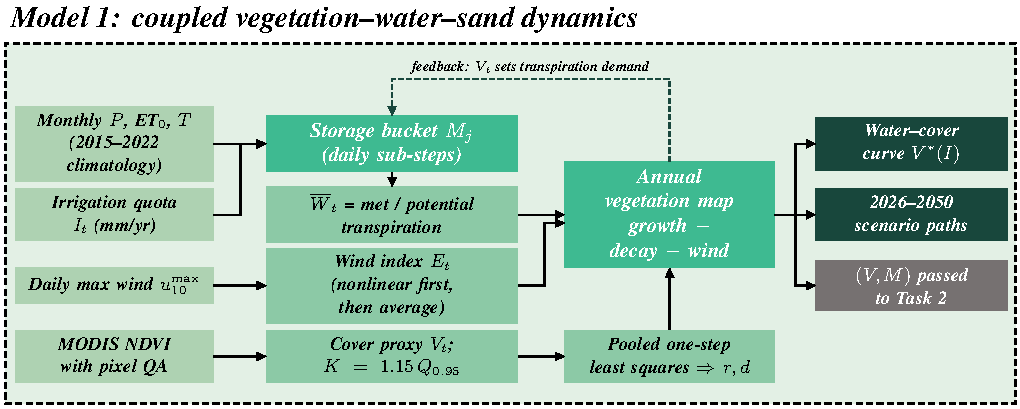
\includegraphics[width=\textwidth]{m1_structure.pdf}
\caption{Structure of Model 1. Inputs on the left; the storage bucket runs on daily sub-steps
inside each year; the vegetation map updates once per year; outputs on the right.}
\label{fig:struct}
\end{figure}

\paragraph{Two states, two time scales.}
\begin{itemize}
\item $V_t$ (yearly): mean NDVI-derived cover proxy of the June--September growing season of year $t$,
with end-members NDVI $0.05$ (bare) and $0.85$ (full): $V=100\,\mathrm{clip}\big((\mathrm{NDVI}-0.05)/0.80,0,1\big)$.
\item $M_j$ (daily sub-steps $j$ within each year, carried across years): water above wilting point in the root zone, $0\le M_j\le C$.
\end{itemize}

\paragraph{Order of computation in each year.}
(1) Hold $V_t$ fixed; (2) run the storage bucket over every day of the year with that year's rain,
ET$_0$ and irrigation; (3) sum transpiration into the met-demand ratio $\Wb_t$;
(4) update $V_{t+1}$ with $\Wb_t$ and the wind index $E_t$; (5) carry the year-end storage to next year.

\paragraph{Three processes in the vegetation equation.}
Logistic growth limited by water and a local ceiling $K$; first-order natural decay; wind damage that
weakens as cover increases (shading).

\paragraph{Four feedback links.}
water $\to$ vegetation (growth is multiplied by $\Wb$);
vegetation $\to$ water (more cover means more transpiration demand, so lower $\Wb$);
vegetation $\to$ sand (shading factor $1-\eta V/K$);
sand $\to$ vegetation (wind damage $kE_{\mathrm{eff}}V$).

\say{Present Fig.~\ref{fig:struct} first, then the vegetation equation, then the bucket. Stress
that $\Wb$ is a transpiration ratio, not soil moisture; $M$ is the soil-water state.}

% =====================================================================
\section{Formulas and what they mean}\label{sec:eq}

\subsection{Vegetation update (yearly)}
\begin{equation}\label{eq:veg}
V_{t+1}=V_t+\underbrace{rV_t\Big(1-\frac{V_t}{K}\Big)\Wb_t}_{\text{growth}}
-\underbrace{dV_t}_{\text{natural decay}}
-\underbrace{kE_t\Big(1-\eta\frac{V_t}{K}\Big)V_t}_{\text{wind damage}}
\end{equation}
\begin{itemize}
\item \textbf{Growth.} $rV$ is exponential growth; $(1-V/K)$ stops growth at the local ceiling $K$;
$\Wb_t\in[0,1]$ scales growth by how much of the plants' water demand was met. Temperature is
already inside $r$ (one yearly growth season), so no extra temperature factor is multiplied here.
\item \textbf{Decay.} A fixed share $d$ of cover dies each year. With no water and no wind,
$V_{t+1}=(1-d)V_t$, so the half-life is $\ln(1/2)/\ln(1-d)$ years.
\item \textbf{Wind damage.} Loss proportional to cover and to the wind index $E_t$; the factor
$(1-\eta V/K)$ means denser cover shelters itself ($\eta=1$: full shelter at $V=K$).
\item $V=0$ stays at 0: water alone cannot create plants; new stands need a planted initial cover.
\end{itemize}

\subsection{Effective soil-water storage (daily sub-steps)}
Monthly rain $P$, ET$_0$ and the month's share of irrigation are spread evenly over the days of that month.
Potential transpiration on day $j$:
\begin{equation}\label{eq:demand}
D_j=c\,\min(1,2f_{c,t})\,f(T_j)\,\mathrm{ET}_{0,j},\qquad f_{c,t}=\mathrm{clip}(V_t/V_{\mathrm{full}},0,1).
\end{equation}
Demand grows with cover until $V$ reaches half of $V_{\mathrm{full}}$, and follows the season through $f(T)$.
Yearly irrigation $I_t$ is split over months in proportion to $f(T)\mathrm{ET}_0$ (watering follows demand).
\begin{align}
B_j&=M_j+\alpha_PP_j+\eta_wI_j+G_j &&\text{water available today}\label{eq:avail}\\
Q_j&=\max(B_j-C,0) &&\text{overflow to deep drainage}\notag\\
K_{s,j}&=\min\{1,\ (B_j-Q_j)/[(1-p)C]\} &&\text{FAO-56 stress coefficient}\notag\\
T_{a,j}&=\min(B_j-Q_j,\ K_{s,j}D_j) &&\text{actual transpiration}\notag\\
M_{j+1}&=B_j-Q_j-T_{a,j} &&\text{storage carried to next day}\label{eq:store}\\
\Wb_t&=\textstyle\sum_{j\in t}T_{a,j}\big/\sum_{j\in t}D_j &&\text{share of demand met in year }t\label{eq:wbar}
\end{align}
Every step conserves water exactly: $M_{j+1}-M_j=\alpha_PP_j+\eta_wI_j+G_j-T_{a,j}-Q_j$.
\begin{itemize}
\item $\alpha_P$ and $\eta_w$ are the shares of rain and of gross irrigation that reach the roots;
interception, soil evaporation and conveyance losses are inside them.
\item Plants are unstressed while storage is above $(1-p)C$; below that, transpiration falls linearly.
\item When storage is full, extra water drains ($Q_j$) and does not raise $\Wb$.
\end{itemize}

\subsection{Helper relations}
\begin{align}
f(T)&=\min\{1,\max\{0,(T-5)/20\}\} &&\text{0 below 5\,$^\circ$C, 1 above 25\,$^\circ$C}\label{eq:fT}\\
q_i&=u_i^2\max(u_i-u_T,0),\ \ u_T=5\ \mathrm{m/s} &&\text{daily sand-drift proxy from daily max wind}\label{eq:q}\\
E_t&=\frac{\tfrac1{n_t}\sum_{i\in t}q_i/\bar q}{\text{training-period mean of the same}} &&\text{wind index, 1 = training mean}\label{eq:E}\\
K&=1.15\times Q_{0.95}(V_{\text{train}}) &&\text{local ceiling from the 95th percentile}\label{eq:K}
\end{align}
The wind proxy is computed on each day and averaged afterwards; averaging the wind first would
hide most gusts above the 5 m/s threshold and make $E$ almost zero.

\subsection{Long-run state and the closed form}
With $x=V/K$ and $\Wb$, $E$ held fixed, the non-zero steady state is
\begin{equation}\label{eq:xstar}
x^*=\frac{r\Wb-d-kE}{r\Wb-kE\eta},\qquad\text{exists if } r\Wb>d+kE.
\end{equation}
Because $\Wb$ itself depends on $V$, the real long-run state is the fixed point of the yearly map
$(V,M)\mapsto(V',M')$, found by iterating from a low and a high start until both agree
(residual $<10^{-7}$). With ample water ($\Wb=1$) and $k=0$: $x^*=1-d/r=0.804$, i.e.\ $V^*=30.6\%$
at $K=38.08\%$, which is exactly the saturation value found numerically.

\subsection{Calibration and checks}
\begin{equation}\label{eq:obj}
\min_{r,d}\ \frac1N\sum_{(s,t)\in\text{train}}\Big(\tilde x_{s,t}\big[1+r(1-\tilde x_{s,t})-d\big]-\tilde x_{s,t+1}\Big)^2
\end{equation}
One-step transitions at 7 irrigated oasis stations, pooled, assuming $\Wb=1$ and $k=0$ there;
training = target year $\le2022$ (49 transitions), hold-out = 2023--2025 (21 transitions).
The residual is linear in $(r,d)$, so the least-squares solution is unique.
Uncertainty: local covariance, leave-one-station-out, and 300 whole-station bootstrap resamples.
Skill: RMSE in $x=V/K$, compared with persistence ($\hat x_{t+1}=x_t$) and the training-period station mean.

\say{Explain why $r,d$ are fitted only at oases: there $\Wb\approx1$, so growth and decay can be
separated from water. If you fit free $r,d,K$ on a planted section, only $r-d$ and $r/K$ are identifiable.}

% =====================================================================
\section{Algorithms}\label{sec:alg}

Model 1 uses four algorithms: prepare the data (Alg.~\ref{alg:prep}), fit $r,d$ (Alg.~\ref{alg:cal}),
step the coupled system through one year (Alg.~\ref{alg:year}), and find the long-run state (Alg.~\ref{alg:scen}).
Thresholds and settings are listed in Section~\ref{sec:par}; the algorithms show only the logic.

\begin{algorithm}[H]
\caption{Data preparation}\label{alg:prep}
\begin{algorithmic}[1]
\Require NDVI time series with pixel quality flags, for each station
\Ensure relative cover $x_{s,t}$; training and hold-out pairs
\State Keep only reliable pixels; build yearly growing-season cover $V_{s,t}$ (missing years stay missing)
\State $K_s\gets1.15\,Q_{0.95}$ of station $s$'s training-period cover \Comment{Eq.~\eqref{eq:K}}
\State $x_{s,t}\gets V_{s,t}/K_s$
\State Split consecutive-year pairs $(x_{s,t},x_{s,t+1})$ by target year into training and hold-out sets
\end{algorithmic}
\end{algorithm}

\begin{algorithm}[H]
\caption{Calibration of $r,d$: pooled linear least squares}\label{alg:cal}
\begin{algorithmic}[1]
\Require training pairs from Alg.~\ref{alg:prep}
\Ensure $\hat r,\hat d$ and their uncertainty
\State \textbf{Linearise.} With $\Wb=1$, $k=0$, Eq.~\eqref{eq:veg} becomes
$\underbrace{x_{t+1}-x_t}_{y}=r\,\underbrace{x_t(1-x_t)}_{z_1}-d\,\underbrace{x_t}_{z_2}$
\State Stack all stations' pairs: $\bm y$ and $\bm Z=[\bm z_1,\ -\bm z_2]$
\State \textbf{Solve} $(\hat r,\hat d)^\top=(\bm Z^\top\bm Z)^{-1}\bm Z^\top\bm y$ \Comment{unique; Eq.~\eqref{eq:obj}}
\State \textbf{Uncertainty:} refit on resampled \emph{whole stations} (cluster bootstrap)
\State \textbf{Check:} one-step error on hold-out pairs vs persistence $\hat x_{t+1}=x_t$
\end{algorithmic}
\end{algorithm}
\noindent\textbf{Key point.} Fixing $K$ beforehand makes the model linear in $(r,d)$, so the fit is an ordinary
regression with one exact answer. $r$ and $d$ are told apart because growth $x(1-x)$ peaks at medium cover
while decay $x$ keeps rising.

\begin{algorithm}[H]
\caption{One model year: water storage drives vegetation}\label{alg:year}
\begin{algorithmic}[1]
\Require cover $V_t$, storage $M$, irrigation $I_t$, one year of daily rain, ET$_0$, temperature
\Ensure $V_{t+1}$, $M$ at year end, $\Wb_t$
\State Demand $D_j$ from current cover and season \Comment{Eq.~\eqref{eq:demand}; $V_t$ held fixed}
\For{each day $j$}
  \State $M\gets M+$ effective rain $+$ effective irrigation
  \State Spill $M-C$ if storage is over capacity \Comment{drainage}
  \State Transpire $T_{a,j}=\min(M,\,K_s(M)\,D_j)$;\quad $M\gets M-T_{a,j}$ \Comment{stress when storage is low}
\EndFor
\State $\Wb_t\gets\sum_jT_{a,j}/\sum_jD_j$ \Comment{share of demand met}
\State $V_{t+1}\gets$ Eq.~\eqref{eq:veg} with $\Wb_t$
\State \Return $V_{t+1}$, $M$ (carried to next year), $\Wb_t$
\end{algorithmic}
\end{algorithm}
\noindent\textbf{Key point.} Water reaches vegetation only through storage: it carries over between days and
years, overflow is lost, and growth uses the \emph{share of demand met}, not the amount applied. Cover feeds back
by setting the demand. Every day conserves water exactly (Eq.~\eqref{eq:store}).

\noindent\textbf{Mathematical tools.} (i) An explicit daily \emph{mass-balance difference equation} (a ``bucket''
or linear-reservoir model); (ii) \emph{piecewise-linear operators}: $\max(\cdot,0)$ for overflow, the
FAO-56 stress ramp $K_s$, and $\min(\cdot)$ so plants never take more than is stored; (iii) a
\emph{ratio aggregation} $\Wb=\sum T_a/\sum D$ that passes the fast (daily) water state to the slow (yearly)
logistic map. The two time scales are nested: $V$ is frozen within the year, $M$ is updated every day.

\begin{figure}[H]\centering
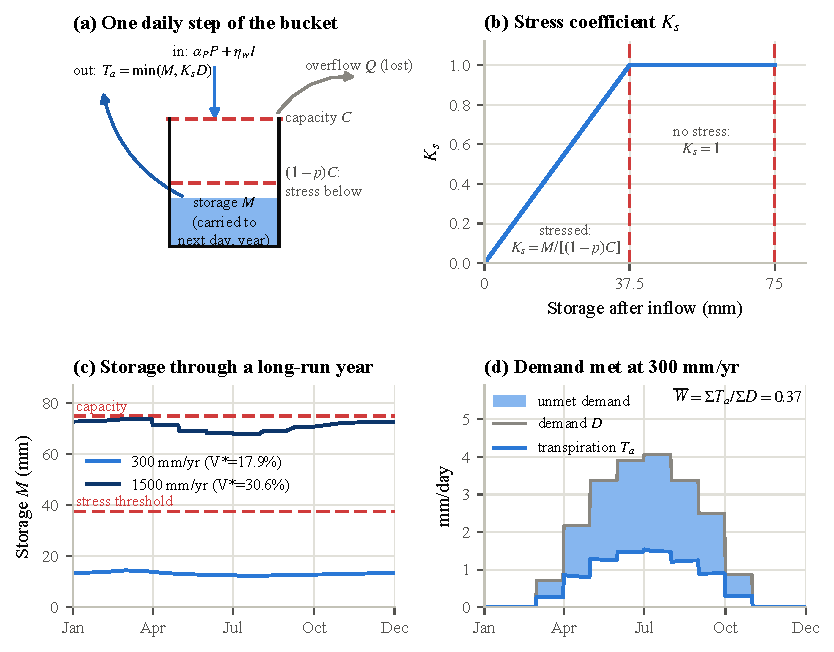
\includegraphics[width=\textwidth]{../../Figures/M1/m1_f10_bucket_mechanism.pdf}
\caption{How Alg.~\ref{alg:year} works. (a) One daily step. (b) The stress ramp: below $(1-p)C=37.5$ mm transpiration
is cut in proportion to storage. (c) Daily storage in a long-run year: at 300 mm/yr storage stays near 13 mm, so plants
are stressed all year; at 1,500 mm/yr storage stays near capacity and 43.5 mm/yr overflows. (d) At 300 mm/yr only 37\%
of demand is met ($\Wb=0.37$), which is what limits cover to 17.9\%.}
\label{fig:bucket}
\end{figure}

\begin{algorithm}[H]
\caption{Long-run state for a given irrigation level}\label{alg:scen}
\begin{algorithmic}[1]
\Require irrigation $I$; a repeated typical climate year
\Ensure long-run $(V^*,M^*,\Wb^*)$
\For{a low and a high starting cover}
  \Repeat\ apply Alg.~\ref{alg:year}
  \Until{$V$ and $M$ stop changing}
\EndFor
\State Accept only if both starts reach the same point
\end{algorithmic}
\end{algorithm}
\noindent\textbf{Key point.} Because $\Wb$ depends on $V$, the closed form Eq.~\eqref{eq:xstar} is only conditional;
the long-run state is the fixed point of the coupled yearly map. Repeating Alg.~\ref{alg:year} over many years
from a planted start gives the scenario paths; varying one parameter gives the sensitivity table.

\noindent\textit{Code:} Alg.~\ref{alg:prep}--\ref{alg:cal}: \texttt{Code/v7\_model1.py} (\texttt{yearly\_table},
\texttt{fit\_stations}), \texttt{Code/v7\_m1\_run.py} (\texttt{bootstrap});
Alg.~\ref{alg:year}--\ref{alg:scen}: \texttt{Code/v7\_m1\_water.py} (\texttt{water\_year}, \texttt{equilibrium}, \texttt{trajectory}).

% =====================================================================
\section{Parameters}\label{sec:par}

\begin{table}[H]\centering\small
\begin{tabularx}{\textwidth}{@{}l l l Y@{}}
\toprule
Symbol & Value (range tested) & Unit & Meaning and status \\
\midrule
$r$ & 0.547 (bootstrap 95\%: 0.335--1.168) & yr$^{-1}$ & intrinsic growth rate; fitted \\
$d$ & 0.107 (bootstrap 95\%: 0.077--0.202) & yr$^{-1}$ & natural decay rate; fitted \\
$K$ & 38.08 (section); per station $1.15Q_{0.95}$ & \% & cover ceiling; rule from data \\
$k$ & 0 (0, 0.02, 0.05, 0.10) & -- & wind damage; scenario (fit not identifiable) \\
$\eta$ & 1 & -- & shading strength; scenario \\
$C$ & 75 (30--150) & mm & storage capacity; scenario \\
$p$ & 0.5 (0.3--0.7) & -- & stress-free share of storage (FAO-56); scenario \\
$c$ & 1.0 (0.7--1.2) & -- & transpiration coefficient; scenario \\
$\eta_w$ & 0.75 (0.65--0.85) & -- & share of gross irrigation that reaches roots; scenario \\
$\alpha_P$ & 0.25 (0--1) & -- & share of rain that reaches roots; scenario \\
$G$ & 0 & mm/yr & groundwater supply; scenario \\
$V_{\mathrm{full}}$ & 66.59 (64.85--69.40) & \% & full-cover end-member (local oasis NDVI 0.5827) \\
$u_T$ & 5 & m/s & wind threshold for sand drift \\
$V_0$, $M_0$ & 2, 37.5 & \%, mm & initial state of a new stand in scenarios \\
\bottomrule
\end{tabularx}
\caption{Model 1 parameters. ``Scenario'' means no field data to fit it; values are stated assumptions with tested ranges.}
\label{tab:par}
\end{table}

\paragraph{Data and forcing.}
\begin{itemize}
\item Stations: ALE, KEL, MF, QM, RQ, YL, YT (vegetated; all 7 pass the training missing-data rule).
MODIS 250 m 16-day NDVI, pixel QA 0/1 only, $\ge50\%$ valid pixels per composite, $\ge2$ valid growing-season months per year.
395 of 396 growing-season station-months valid; no interpolated values are used for fitting or scoring.
\item Climate for scenarios: 2015--2022 monthly climatology of Yutian/Minfeng (Open-Meteo archive):
rain 52.2 mm/yr, ET$_0$ 1,685.6 mm/yr, temperature-weighted ET$_0$ 1,190.8 mm/yr; wind index peaks in April (2.29) and May (2.08).
\item Raw MODIS replay: all 198 downloaded chunks match the original SHA-256 hashes.
\end{itemize}

% =====================================================================
\section{Results}

\subsection{Calibration and model selection}
\begin{table}[H]\centering\small
\resizebox{\textwidth}{!}{\begin{tabular}{@{}lcccccc@{}}
\toprule
Model & Parameters & Cond.\ number & AIC & RMSE train & RMSE hold-out & $R^2$ hold-out\\
\midrule
M0 $(r,d)$ \textbf{adopted} & $r=0.547\pm0.174$, $d=0.107\pm0.033$ & 375 & $-286.48$ & 0.0516 & 0.0635 & 0.463\\
M1 $(+k)$ & $r=0.778$, $d=0.105$, $k=0.249\pm0.431$ & 4,406 & $-284.83$ & 0.0514 & 0.0657 & 0.424\\
M2 $(+k,\eta)$ & same, $\eta=1.0$ at bound & 94,351 & $-282.83$ & 0.0514 & 0.0657 & 0.424\\
\midrule
Persistence & $\hat x_{t+1}=x_t$ & -- & -- & 0.0572 & \textbf{0.0536} & --\\
Station mean & training mean & -- & -- & -- & 0.0737 & --\\
\bottomrule
\end{tabular}}
\caption{Nested fits (units of $x=V/K$). Adding wind damage worsens AIC and hold-out error and the
uncertainty of $k$ exceeds its value, so $k$ is kept as a scenario parameter.}
\label{tab:fit}
\end{table}
\begin{itemize}
\item Hold-out skill by station (MSE skill vs persistence): MF $+0.44$, YT $+0.20$; ALE $-0.44$, RQ $-0.52$, YL $-0.57$, KEL $-2.62$, QM $-2.88$.
\item Leave-one-station-out: $r$ stays in 0.47--0.53 and $d$ in 0.09--0.11 for six stations; leaving out YT gives $r=0.958$, $d=0.168$ (YT is influential).
\item Bootstrap (300 resamples of whole stations, only 7 clusters): $r$ median 0.554, 95\% 0.335--1.168; $d$ median 0.109, 95\% 0.077--0.202.
\item Stricter QA (75\% valid pixels, 6 stations): $r=0.510$, $d=0.103$; conclusions unchanged.
\item Free run from 2022 to 2025: the model stays near 2022 values while most stations greened in 2023--2025
(e.g.\ RQ predicted 33.0\% vs observed 38.4\% in 2025; QM 30.7\% vs 37.2\%).
\item Section pixels (retrospective): station parameters transferred to planted pixels of CON1--3 give $R^2=0.398$
(RMSE 8.1 points, $n=116$); CON4 gives $R^2=0.318$ (RMSE 12.1 points, $n=129$). A free fit there gives net rate $r-d=0.543$ and plateau 35.3\%.
\item Water bookkeeping: largest balance error over all scenarios $5.3\times10^{-13}$ mm. No-water half-life: 6.1 years.
\end{itemize}

\subsection{Irrigation--cover curve (long-run state)}
\begin{table}[H]\centering\small
\begin{tabular}{@{}rrrrrr@{}}
\toprule
Irrigation (mm/yr) & m$^3$/ha/yr & $V^*$ (\%) & $M^*$ end of year (mm) & $\Wb^*$ & Relative erosion $1-\eta V^*/K$\\
\midrule
0 & 0 & 1.77 & 7.1 & 0.21 & 0.95\\
50 & 500 & 6.05 & 8.3 & 0.23 & 0.84\\
100 & 1,000 & 9.43 & 9.4 & 0.26 & 0.75\\
150 & 1,500 & 12.17 & 10.5 & 0.29 & 0.68\\
200 & 2,000 & 14.43 & 11.5 & 0.32 & 0.62\\
300 & 3,000 & 17.94 & 13.4 & 0.37 & 0.53\\
400 & 4,000 & 20.54 & 15.4 & 0.43 & 0.46\\
500 & 5,000 & 22.54 & 17.3 & 0.48 & 0.41\\
600 & 6,000 & 24.14 & 19.3 & 0.54 & 0.37\\
800 & 8,000 & 26.51 & 23.2 & 0.65 & 0.30\\
1,000 & 10,000 & 28.20 & 27.0 & 0.76 & 0.26\\
1,500 & 15,000 & 30.60 & 72.8 & 1.00 & 0.20\\
2,000 & 20,000 & 30.60 & 74.4 & 1.00 & 0.20\\
\bottomrule
\end{tabular}
\caption{Long-run state for constant irrigation (fixed point, converged from both starts). The last column is the shading factor, not a measured erosion reduction.}
\label{tab:curve}
\end{table}
\begin{itemize}
\item \textbf{Diminishing returns.} The first 100 mm/yr adds 7.7 points of cover (0.077 points per mm);
500$\to$600 mm adds 1.6 points (0.016 per mm); 800$\to$1,000 mm adds 1.7 points (0.008 per mm).
\item \textbf{Saturation.} Above about 1,500 mm/yr, $\Wb=1$, storage is full and the extra water drains; cover is capped at $K(1-d/r)=30.6\%$.
\item \textbf{Rain alone} (52 mm/yr) holds only 1.8\% cover.
\end{itemize}

\subsection{Scenario paths 2026--2050}
Start: $V_0=2\%$, $M_0=37.5$ mm; climate repeats the 2015--2022 average year (not a weather forecast).
\begin{table}[H]\centering\small
\begin{tabular}{@{}lrrrrr@{}}
\toprule
Scenario & 2030 & 2035 & 2036 & 2040 & 2050\\
\midrule
No irrigation & 2.19 & 1.99 & 1.97 & 1.89 & 1.80\\
100 mm/yr & 6.25 & 7.99 & 8.20 & 8.78 & 9.30\\
300 mm/yr & 9.90 & 15.50 & 16.00 & 17.16 & 17.86\\
600 mm/yr & 9.90 & 21.53 & 22.31 & 23.69 & 24.13\\
1,000 mm/yr & 9.90 & 25.15 & 26.43 & 27.99 & 28.20\\
600 mm/yr, stopped after 2035 & 9.90 & 21.53 & 19.46 & 12.74 & 5.09\\
\bottomrule
\end{tabular}
\caption{Cover proxy $V$ (\%) at the end of each year.}
\label{tab:scen}
\end{table}
\begin{itemize}
\item \textbf{Establishment is growth-limited.} Every quota of 300 mm/yr or more gives the same 9.90\% in 2030:
young stands use little water, storage stays full and the surplus drains. Water above $\sim$300 mm/yr is wasted in the first five years.
\item \textbf{Stopping water undoes the work.} After irrigation stops, $\Wb$ falls to 0.03--0.07 and cover drops from 21.5\% to 12.7\% in 5 years and to 5.1\% in 15 years.
\item It takes about 15--25 years to get close to the long-run value (300 mm/yr: 17.86\% in 2050 vs 17.94\% long-run).
\end{itemize}

\subsection{Sensitivity}
\begin{table}[H]\centering\small
\begin{tabular}{@{}llrrrr@{}}
\toprule
Parameter & Low / high & \multicolumn{2}{c}{$V^*$ at 300 mm/yr} & \multicolumn{2}{c}{$V^*$ at 600 mm/yr}\\
 & & low & high & low & high\\
\midrule
Baseline & -- & \multicolumn{2}{c}{17.94} & \multicolumn{2}{c}{24.14}\\
Transpiration coefficient $c$ & 0.7 / 1.2 & 21.32 & 16.22 & 27.12 & 22.49\\
Irrigation efficiency $\eta_w$ & 0.65 / 0.85 & 16.66 & 19.06 & 22.89 & 25.20\\
Rain share $\alpha_P$ & 0 / 1 & 17.40 & 19.38 & 23.89 & 24.85\\
Full-cover end-member $V_{\mathrm{full}}$ & 64.85 / 69.40 & 17.68 & 18.33 & 23.91 & 24.50\\
Storage capacity $C$ & 30 / 150 mm & 17.94 & 17.94 & 24.14 & 24.14\\
Stress share $p$ & 0.3 / 0.7 & 17.94 & 17.94 & 24.14 & 24.14\\
\midrule
Wind damage $k$ (300 mm/yr) & 0 / 0.02 / 0.05 / 0.10 & \multicolumn{4}{l}{17.94 / 17.01 / 15.66 / 13.62}\\
\bottomrule
\end{tabular}
\caption{Long-run cover under one-at-a-time changes.}
\label{tab:sens}
\end{table}
\begin{itemize}
\item The demand side ($c$) and the efficiency of water delivery ($\eta_w$) matter most; each moves $V^*$ by 1--3 points.
\item Storage capacity and $p$ do not change the long-run cover (they change $M$ only). Reason: in a repeating year without
overflow, storage returns to the same value, so yearly transpiration equals yearly effective inflow and
$\Wb$ depends only on inflow and demand. Capacity matters for the timing within the year and for the start-up phase.
\item Wind damage is the largest single uncertainty: $k=0.10$ removes 24\% of the cover at 300 mm/yr.
\end{itemize}

% =====================================================================
\section{What we can claim and what we cannot}
\begin{tabularx}{\textwidth}{@{}YY@{}}
\toprule
Can claim & Must not claim\\
\midrule
A mass-conserving coupled $V$--$M$ model, calibrated on real NDVI with stated assumptions. &
That the water response is field-calibrated (no measured irrigation--storage--cover data). \\
Growth and decay rates with honest, wide uncertainty. &
That the model beats persistence for one-year forecasts (it does not). \\
Irrigation has strongly diminishing returns; establishment needs little water; stopping water causes collapse within $\sim$15 yr. &
Measured ground cover: $V$ is an NDVI proxy; 1 km width and 128 km length are a study scenario, not an engineering boundary. \\
Wind damage could remove up to a quarter of the cover (scenario). &
Erosion reduction in tonnes or percent; CON4 as an independent validation (pixels were selected using later greening). \\
\bottomrule
\end{tabularx}

% =====================================================================
\section{Figures ready for the paper}
\begin{table}[H]\centering\small
\begin{tabularx}{\textwidth}{@{}lY@{}}
\toprule
File (\texttt{Figures/M1/}) & What it shows / caption point\\
\midrule
\texttt{m1\_f01\_station\_series} & 7 stations 2015--2025: observed $V$, one-step prediction, free run from 2022, persistence, local $K$\\
\texttt{m1\_f02\_holdout\_skill} & Observed vs predicted; per-station hold-out RMSE vs persistence (negative skill kept)\\
\texttt{m1\_f03\_parameter\_bootstrap} & $r$--$d$ cloud from bootstrap, leave-one-out points, pooled fit\\
\texttt{m1\_f04\_cohort\_diagnostic} & Planted pixels CON1--4 vs transferred curve (retrospective only)\\
\texttt{m1\_f05\_forcing\_climatology} & Monthly rain, ET$_0$, temperature-weighted ET$_0$, wind index\\
\texttt{m1\_f06\_water\_cover\_curve} & Irrigation vs long-run $V$, $\Wb$, $M$, relative erosion\\
\texttt{m1\_f07\_scenario\_trajectories} & 2026--2050 paths for constant quotas and the stop-after-10 case\\
\texttt{m1\_f08\_monthly\_water\_balance} & Monthly inflow, transpiration, drainage and storage\\
\texttt{m1\_f09\_sensitivity} & Tornado chart of water parameters; wind damage scenarios\\
\bottomrule
\end{tabularx}
\end{table}

\begin{figure}[H]\centering
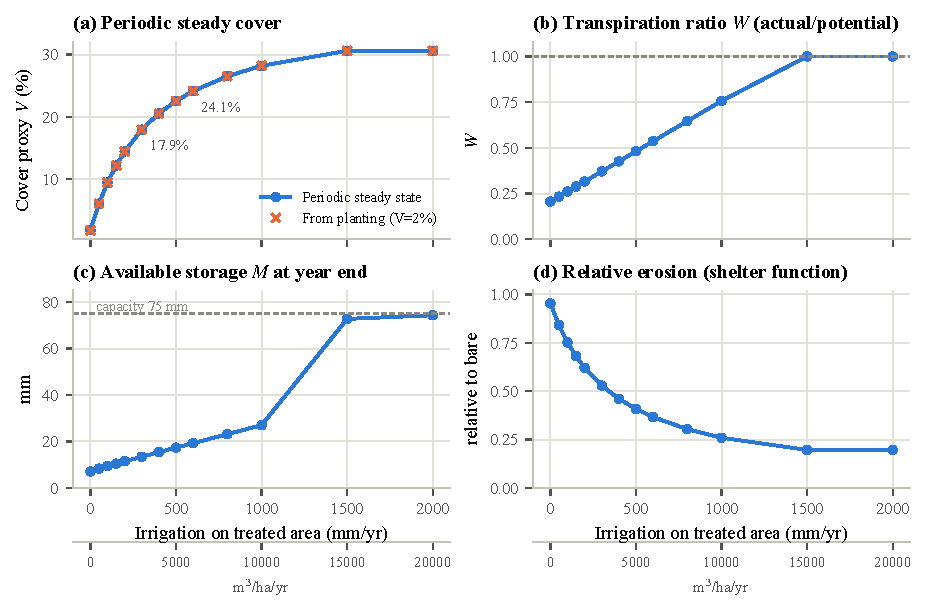
\includegraphics[width=0.92\textwidth]{../../Figures/M1/m1_f06_water_cover_curve.pdf}
\caption{(From \texttt{m1\_f06}) Irrigation--cover curve. Use it for the ``diminishing returns'' and ``saturation'' points.}
\end{figure}

\begin{figure}[H]\centering
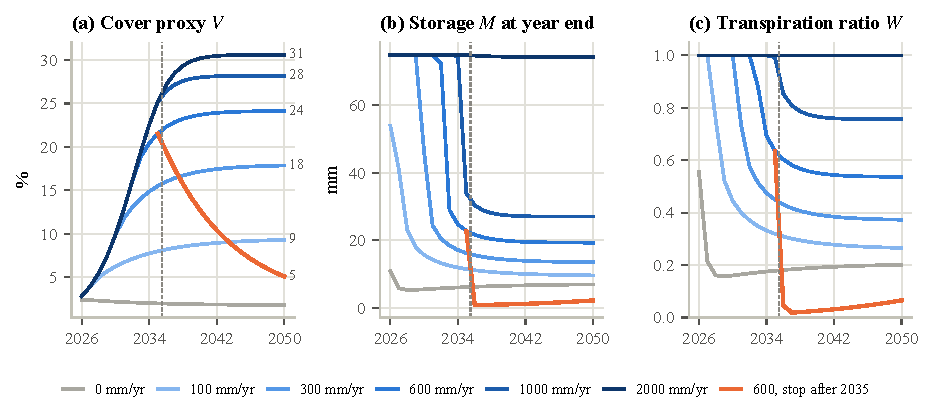
\includegraphics[width=0.92\textwidth]{../../Figures/M1/m1_f07_scenario_trajectories.pdf}
\caption{(From \texttt{m1\_f07}) Scenario paths 2026--2050, including stopping irrigation after 10 years.}
\end{figure}

\section{Suggested outline for the Model 1 section}
\begin{enumerate}
\item Section choice and data (Yutian--Minfeng, 127.95 km $\times$ 1 km scenario; stations; QA rules).
\item Model structure (Fig.~\ref{fig:struct}) and the four feedback links.
\item Equations \eqref{eq:veg}--\eqref{eq:wbar} with one line each on meaning.
\item Algorithms: data preparation (Alg.~\ref{alg:prep}), calibration as linear regression (Alg.~\ref{alg:cal}), one model year (Alg.~\ref{alg:year}), long-run state (Alg.~\ref{alg:scen}).
\item Parameters (Table~\ref{tab:par}); calibration result Table~\ref{tab:fit}, honest skill statement, bootstrap.
\item Results: irrigation--cover curve (Table~\ref{tab:curve}), scenario paths (Table~\ref{tab:scen}).
\item Influencing factors: sensitivity (Table~\ref{tab:sens}), wind damage scenarios.
\item Limits and the hand-over to Model 2: each planted cohort carries its own $(V,M)$.
\end{enumerate}

\end{document}
